\chapter{Conjuntos y Funciones}

Introduciremos en este capítulo el lenguaje de Conjuntos y Funciones, que será utilizado sistemáticamente en los capítulos siguientes. Toda la Matemática se presenta hoy en día en ese lenguaje; así, imaginamos que la mayoría de los lectores ya tenga cierta familiaridad con el tema. Sin embargo, no se exigirá conocimiento previo alguno de la materia.

\section{Conjuntos}

Un conjunto (o colección) está formado por objetos, llamados sus elementos. La relación básica entre un objeto y un conjunto es la relación de pertenencia. Cuando un objeto \( x \) es uno de los elementos que componen el conjunto \( A \), decimos que \( x \) pertenece a \( A \) y escribimos
\[ x \in A. \]

Si, en cambio, \( x \) no es uno de los elementos del conjunto \( A \), decimos que \( x \) no pertenece a \( A \) y escribimos
\[ x \notin A. \]

Un conjunto \( A \) queda definido (o determinado, o caracterizado) cuando se da una regla que permita decidir si un objeto arbitrario \( x \) pertenece o no a \( A \).

Ejemplo 1. Sea \( A \) el conjunto de los triángulos rectángulos. El conjunto \( A \) está bien definido: un objeto \( x \) pertenece a \( A \) cuando es un triángulo y, además, uno de sus ángulos es recto. Si \( x \) no es un triángulo, o si \( x \) es un triángulo que no posee ángulo recto, entonces \( x \) no pertenece a \( A \).

Se usa la notación
\[ X = \{a, b, c, \ldots\} \]
para representar el conjunto \( X \) cuyos elementos son los objetos \( a, b, c \), etc. Así, por ejemplo, \( \{1, 2\} \) es el conjunto cuyos elementos son los números 1 y 2. Dado el objeto \( a \), puede considerarse el conjunto cuyo único elemento es \( a \). Ese conjunto se representa por \( \{a\} \).

El conjunto de los números naturales 1, 2, 3, … será representado por el símbolo \( \mathbb{N} \). Por tanto
\[ \mathbb{N} = \{1, 2, 3, \ldots\}. \]

El conjunto de los números enteros (positivos, negativos y cero) será indicado por el símbolo \( \mathbb{Z} \). Así,
\[ \mathbb{Z} = \{\ldots, -3, -2, -1, 0, 1, 2, 3, \ldots\}. \]

El conjunto \( \mathbb{Q} \), de los números racionales, está formado por las fracciones \( p/q \), donde \( p \) y \( q \) pertenecen a \( \mathbb{Z} \), siendo \( q \neq 0 \). En símbolos,

\[
\mathbb{Q} = \{p/q \; ; \quad p \in \mathbb{Z}, \quad q \in \mathbb{Z}, \quad q \neq 0\}.
\]

Se lee: "\( \mathbb{Q} \) es el conjunto de las fracciones \( p/q \) tales que \( p \) pertenece a \( \mathbb{Z} \), \( q \) pertenece a \( \mathbb{Z} \) y \( q \) es diferente de cero".

La mayoría de los conjuntos encontrados en Matemática no se definen especificando, uno a uno, sus elementos. El método más frecuente para definir un conjunto es mediante una propiedad común y exclusiva de sus elementos. Más precisamente, se parte de una propiedad \( P \). Ella define un conjunto \( X \) así: si un objeto \( x \) goza de la propiedad \( P \), entonces \( x \in X \); si \( x \) no goza de \( P \), entonces \( x \notin X \). Se escribe

\[X = \{x \; ; \quad x \text{ goza de la propiedad } P\}.\]

Se lee: "\( X \) es el conjunto de los elementos \( x \) tales que \( x \) goza de la propiedad \( P \)".

Muchas veces la propiedad \( P \) se refiere a elementos de un conjunto fundamental \( E \). En este caso, se escribe

\[X = \{x \in E \; ; \quad x \text{ goza de la propiedad } P\}.\]

Por ejemplo, sea \( \mathbb{N} \) el conjunto de los números naturales y consideremos la siguiente propiedad, que se refiere a un elemento genérico \( x \in \mathbb{N} \):

"\( x \) es mayor que 5".

La propiedad \( P \), de que un número natural sea mayor que 5, define el conjunto \( X = \{6, 7, 8, 9, \dots\} \), es decir,

\[X = \{x \in \mathbb{N} \; ; \quad x > 5\}.\]

Se lee: "\( X \) es el conjunto de los \( x \) pertenecientes a \( \mathbb{N} \) tales que \( x \) es mayor que 5".

A veces ocurre que ningún elemento de \( E \) goza de la propiedad \( P \). En este caso, el conjunto \( \{x \in E \; ; \quad x \text{ goza de } P\} \) no posee ningún elemento alguno. Esto es lo que se llama un conjunto vacío Para representarlo, usaremos el símbolo \(\emptyset\).

Por lo tanto, el conjunto vacío \(\emptyset\) se define así:

Cualquiera que sea \(x\), se tiene \(x \notin \emptyset\).

Por ejemplo, tenemos \(\{x \in \mathbb{N}; 1 < x < 2\} = \emptyset\). Y también, \(\{x; x \neq x\} = \emptyset\).

Dados los conjuntos \(A\) y \(B\), decimos que \(A\) es subconjunto de \(B\) cuando todo elemento de \(A\) es también elemento de \(B\). Para indicar este hecho, se usa la notación

\[A \subset B.\]

Cuando \(A \subset B\), se dice también que \(A\) es parte de \(B\), que \(A\) está incluido en \(B\), o contenido en \(B\). La relación \(A \subset B\) se llama relación de inclusión.

Ejemplo 2. Los conjuntos numéricos \(\mathbb{N}, \mathbb{Z}\) y \(\mathbb{Q}\), presentados arriba, cumplen las relaciones de inclusión \(\mathbb{N} \subset \mathbb{Z}\) y \(\mathbb{Z} \subset \mathbb{Q}\). Abreviadamente, escribimos \(\mathbb{N} \subset \mathbb{Z} \subset \mathbb{Q}\).

Ejemplo 3. Sean \(X\) el conjunto de los cuadrados e \(Y\) el conjunto de los rectángulos. Todo cuadrado es un rectángulo, luego \(X \subset Y\).

Cuando se escribe \(X \subset Y\) no queda excluida la posibilidad de que resulte \(X = Y\). En el caso en que \(X \subset Y\) y \(X \neq Y\), se dice que \(X\) es una parte propia o un subconjunto propio de \(Y\).

Afirmar \(x \in X\) equivale a afirmar \(\{x\} \subset X\).

Para mostrar que un conjunto \(X\) no es subconjunto de un conjunto \(Y\), se debe obtener un elemento de \(X\) que no pertenezca a \(Y\). Así, por ejemplo, no se tiene \(\mathbb{Q} \subset \mathbb{Z}\), pues \(1/2 \in \mathbb{Q}\) y \(1/2\) no es entero.

De ello se sigue que el conjunto vacío \(\emptyset\) es subconjunto de cualquier conjunto \(X\). En efecto, si no fuera \(\emptyset \subset X\), existiría algún \(x \in \emptyset\) tal que \(x \notin X\). Como no existe \(x \in \emptyset\), estamos obligados a admitir que

\[\emptyset \subset X,\]

sea cual sea el conjunto \(X\).

La relación de inclusión \(A \subset B\) es:

- Reflexiva – \(A \subset A\), sea cual sea el conjunto \(A\);\\
- Antisimétrica – si \(A \subset B\) y \(B \subset A\), entonces \(A = B\);\\
- Transitiva – si \(A \subset B\) y \(B \subset C\), entonces \(A \subset C\).

La verificación de estos tres hechos es inmediata.

Se sigue de la propiedad antisimétrica que dos conjuntos \(A\) y \(B\) son iguales precisamente cuando \(A \subset B\) y \(B \subset A\), es decir, cuando poseen los mismos elementos.

Recordemos que, sean cuales fueren los significados de los símbolos \(E\) y \(D\), el signo de igualdad en una expresión como \(E = D\) significa que los símbolos \(E\) y \(D\) están siendo usados para representar el mismo objeto. En otras palabras, una cosa solo es igual a sí misma.

En el caso de conjuntos, escribir \(A = B\) significa que \(A\) y \(B\) son el mismo conjunto, o sea, que \(A\) y \(B\) poseen los mismos elementos. Siempre que tengamos que probar una igualdad entre conjuntos \(A\) y \(B\), debemos demostrar primero que \(A \subset B\) (esto es, que todo elemento de \(A\) pertenece necesariamente a \(B\)) y, después, que \(B \subset A\).

Dado un conjunto \(X\), se indica con \(\mathcal{P}(X)\) el conjunto cuyos elementos son las partes de \(X\). En otras palabras, afirmar que \(A \in \mathcal{P}(X)\) es lo mismo que decir \(A \subset X\). \(\mathcal{P}(X)\) se llama el conjunto de las partes de \(X\). Nunca es vacío: se tiene al menos \(\emptyset \in \mathcal{P}(X)\) y \(X \in \mathcal{P}(X)\).

Ejemplo 4. Sea \(X = \{1, 2, 3\}\). Entonces

\[
\mathcal{P}(X) = \{\emptyset, \{1\}, \{2\}, \{3\}, \{1, 2\}, \{1, 3\}, \{2, 3\}, X\}.
\]

Sean \(P\) y \(Q\) propiedades que se refieren a elementos de un cierto conjunto \(E\). Las propiedades \(P\) y \(Q\) definen subconjuntos \(X\) e \(Y\) de \(E\), a saber:

\[
X = \{x \in E \; ; \quad x \text{ goza de } P\} \quad \text{y} \quad Y = \{y \in E \; ; \quad y \text{ goza de } Q\}.
\]

Las afirmaciones "P implica Q", "si P, entonces Q", "P acarrea Q", "P es condición suficiente para Q", "Q es condición necesaria para P" tienen todas el mismo significado. Quieren decir que \(X \subset Y\), es decir, que todo objeto que goza de P también goza de Q. Para expresar este hecho, se usa la notación

\[
P \Rightarrow Q.
\]

También las afirmaciones "P si, y solo si, Q", "P es condición necesaria y suficiente para Q" tienen todas el mismo significado. Quieren decir que \(P \Rightarrow Q\) y \(Q \Rightarrow P\), o sea, que el conjunto \(X\) de los elementos que gozan de la propiedad \(P\) coincide con el conjunto \(Y\) de los elementos que gozan de \(Q\). La notación que expresa este hecho es

\[
P \Leftrightarrow Q.
\]

\section{Operaciones entre conjuntos}

La unión de los conjuntos \(A\) y \(B\) es el conjunto \(A \cup B\), formado por los elementos de \(A\) más los elementos de \(B\). Así, afirmar que \(x \in A \cup B\) significa decir que al menos una de las siguientes afirmaciones es verdadera: \(x \in A\) o \(x \in B\). Podemos entonces escribir:

\[
A \cup B = \{x \; ; \quad x \in A \text{ o } x \in B\}.
\]

Al contrario del lenguaje vulgar, la palabra "o" se utiliza siempre en Matemáticas en el sentido amplio: al decir "\(x \in A\) o \(x \in B\)" se quiere afirmar que al menos una de esas dos alternativas es verdadera, sin quedar excluida la posibilidad de que ambas lo sean, es decir, de tenerse al mismo tiempo \(x \in A\) y \(x \in B\).

\begin{center}
    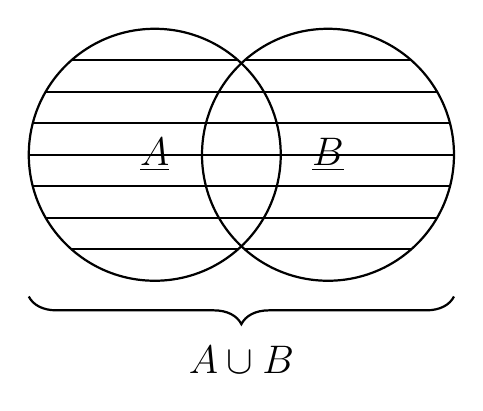
\begin{tikzpicture}[node distance=2.5cm, thick]
        
        \def\radius{1.6}
        \def\dist{1.1}
        
        \begin{scope}
            \clip (-\dist, 0) circle (\radius) (\dist, 0) circle (\radius);
            \foreach \y in {-1.6,-1.2,...,1.6}
                \draw (-\dist-\radius, \y) -- (\dist+\radius, \y);
        \end{scope}

        \draw (-\dist, 0) circle (\radius);
        \draw (\dist, 0) circle (\radius);

        \node at (-\dist, 0) {\Large $\underline{A}$};
        \node at (\dist, 0) {\Large $\underline{B}$};

        \draw [decorate, decoration={brace, mirror, amplitude=10pt}] 
            (-\dist-\radius, -1.8) -- (\dist+\radius, -1.8) 
            node [midway, yshift=-0.8cm] {\Large $A \cup B$};

    \end{tikzpicture}
\end{center}

En la figura anterior, donde \(A\) y \(B\) son discos, la unión \(A \cup B\) es la parte sombreada.

Sean cuales fueren los conjuntos \(A\) y \(B\), se tiene \(A \subset A \cup B\) y \(B \subset A \cup B\).

La intersección de los conjuntos \(A\) y \(B\) es el conjunto \(A \cap B\), formado por los elementos comunes a \(A\) y \(B\). Así, afirmar que \(x \in A \cap B\) significa decir que se tiene, al mismo tiempo, \(x \in A\) y \(x \in B\). Escribimos entonces

\[
A \cap B = \{x \; ; \quad x \in A \text{ y } x \in B\}.
\]

Puede ocurrir que no exista elemento alguno \(x\) tal que \(x \in A\) y \(x \in B\). En este caso, se tiene \(A \cap B = \emptyset\) y los conjuntos \(A\) y \(B\) se dicen disjuntos.

\begin{center}
  \centering
  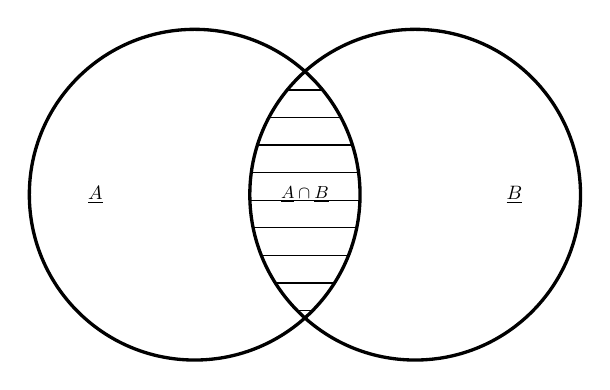
\begin{tikzpicture}[scale=0.7, transform shape, line width=1.2pt]

    \coordinate (A) at (-2,0);
    \coordinate (B) at (2,0);
    \def\rad{3.0}

    \begin{scope}
      \clip (A) circle (\rad);
      \clip (B) circle (\rad);
      
      \foreach \y in {-2.6, -2.1, ..., 2.6} {
        \draw[thin, line width=0.5pt, black] (-4, \y) -- (4, \y);
      }
    \end{scope}

    \draw (A) circle (\rad);
    \draw (B) circle (\rad);

    \node at (-3.8, 0) {\normalsize \(\underline{A}\)};
    \node at (3.8, 0) {\normalsize \(\underline{B}\)};
    
    \node at (0, 0) {\small \(\underline{A} \cap \underline{B}\)};

  \end{tikzpicture}
\end{center}

En la figura anterior, los conjuntos \(A\) y \(B\) están representados por discos y la intersección \(A \cap B\) es la parte sombreada.

Cualesquiera que sean los conjuntos \(A\) y \(B\) se tiene \(A \cap B \subset A\) y \(A \cap B \subset B\).

Ejemplo 5. Sean \(A = \{x \in \mathbb{N}; x \leq 10\}\) y \(B = \{x \in \mathbb{N}; x > 5\}\). Entonces \(A \cup B = \mathbb{N}\) y \(A \cap B = \{6, 7, 8, 9, 10\}\).

Ejemplo 6. Sean \(A = \{x \in \mathbb{N}; x > 2\}\) el conjunto de los números naturales mayores que 2, y \(B = \{x \in \mathbb{N}; x < 3\}\) el conjunto de los números naturales menores que 3. Entonces \(A \cap B = \emptyset\), pues no existen números naturales \(x\) tales que \(2 < x < 3\). Así los conjuntos \(A\) y \(B\) son disjuntos.

Relacionamos en las listas siguientes las principales propiedades formales de las operaciones de unión e intersección.

U1) \(A \cup \emptyset = A\)  \\
U2) \(A \cup A = A\)  \\
U3) \(A \cup B = B \cup A\)  \\
U4) \((A \cup B) \cup C = A \cup (B \cup C)\)  \\
U5) \(A \cup B = A \iff B \subset A\)  \\
U6) \(A \subset B,\; A' \subset B' \Rightarrow A \cup A' \subset B \cup B'\)  \\
U7) \(A \cup (B \cap C) = (A \cup B) \cap (A \cup C)\)

I1) \(A \cap \emptyset = \emptyset\)  \\
I2) \(A \cap A = A\)  \\
I3) \(A \cap B = B \cap A\)  \\
I4) \((A \cap B) \cap C = A \cap (B \cap C)\)  \\
I5) \(A \cap B = A \iff A \subset B\)  \\
I6) \(A \subset B,\; A' \subset B' \Rightarrow A \cap A' \subset B \cap B'\)  \\
I7) \(A \cap (B \cup C) = (A \cap B) \cup (A \cap C)\)

La demostración de cualquiera de estas propiedades se reduce al manejo adecuado de los conectivos "y" y "o". En realidad, podemos interpretar las propiedades anteriores como reglas formales para el manejo de esos conectivos. Demostremos una de ellas, a modo de ejemplo.

Vamos a demostrar ahora U7. Primeramente probaremos que \(A \cup (B \cap C) \subset (A \cup B) \cap (A \cup C)\). Dado \(x \in A \cup (B \cap C)\), se tiene \(x \in A\) o, entonces, \(x \in B \cap C\). En el primer caso, viene \(x \in A \cup B\) y \(x \in A \cup C\), de donde \(x \in (A \cup B) \cap (A \cup C)\). En el segundo caso tenemos \(x \in B\) y \(x \in C\). De \(x \in B\) se sigue \(x \in A \cup B\) y de \(x \in C\) se concluye \(x \in A \cup C\). Luego, \(x \in A \cup B\) y \(x \in A \cup C\), es decir, \(x \in (A \cup B) \cap (A \cup C)\). En cualquier hipótesis, \(x \in A \cup (B \cap C)\) implica \(x \in (A \cup B) \cap (A \cup C)\). Esto quiere decir: \(A \cup (B \cap C) \subset (A \cup B) \cap (A \cup C)\). Ahora mostraremos que \((A \cup B) \cap (A \cup C) \subset A \cup (B \cap C)\). Para esto, sea \(x \in (A \cup B) \cap (A \cup C)\). Entonces \(x \in A \cup B\) y \(x \in A \cup C\). Dentro de esta situación, hay dos posibilidades: o \(x \in A\) o \(x \notin A\). Si \(x \notin A\), entonces (como \(x \in A \cup B\) y \(x \in A \cup C\)) debe ser \(x \in B\) y \(x \in C\), esto es, \(x \in B \cap C\) y, por tanto, \(x \in A \cup (B \cap C)\). Si \(x \in A\) entonces evidentemente \(x \in A \cup (B \cap C)\). En cualquier hipótesis, \(x \in (A \cup B) \cap (A \cup C)\) implica \(x \in A \cup (B \cap C)\), o sea, \((A \cup B) \cap (A \cup C) \subset A \cup (B \cap C)\), como queríamos probar.

La diferencia entre los conjuntos \(A\) y \(B\) es el conjunto \(A - B\), formado por los elementos de \(A\) que no pertenecen a \(B\). En símbolos:

\[
A - B = \{x \; ; \quad x \in A \text{ y } x \notin B\}.
\]

\begin{center}
  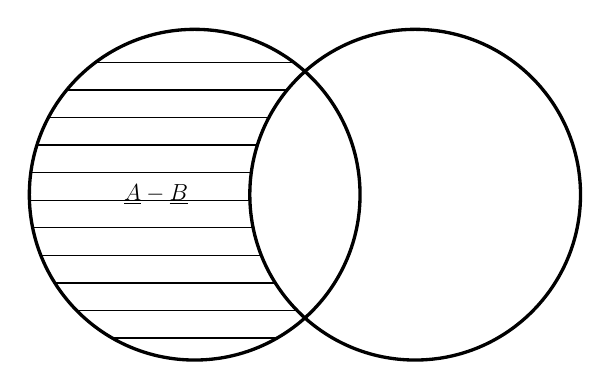
\begin{tikzpicture}[scale=0.7, transform shape, line width=1.2pt]

    \coordinate (A) at (-2,0);
    \coordinate (B) at (2,0);
    \def\rad{3.0}

    \begin{scope}
      \clip (A) circle (\rad);
      
      \foreach \y in {-2.6, -2.1, ..., 2.6} {
        \draw[thin, line width=0.5pt, black] (-5.2, \y) -- (1, \y);
      }
      
      \fill[white] (B) circle (\rad);
    \end{scope}

    \draw (A) circle (\rad);
    \draw (B) circle (\rad);

    \node at (-2.7, 0) {\large \(\underline{A} - \underline{B}\)};

  \end{tikzpicture}
\end{center}

En la figura anterior, donde los conjuntos \(A\) y \(B\) están representados por discos, la diferencia \(A - B\) es la parte sombreada.

No se exige que \(B\) esté contenido en \(A\) para formar la diferencia \(A - B\). Cuando \(A\) y \(B\) son disjuntos, ningún elemento de \(A\) pertenece a \(B\); por tanto, \(A - B = A\). En cualquier caso, se tiene \(A - B = A - (A \cap B)\).

Cuando se tiene \(B \subset A\), la diferencia \(A - B\) se llama el complementario de \(B\) en relación con \(A\) y se escribe

\[
A - B = \mathcal{C}_A B.
\]

Frecuentemente, se tiene un conjunto \(E\) que contiene todos los conjuntos que ocurren en una cierta discusión. En este caso, la diferencia \(E - X\) se llama simplemente el complementario de \(X\) y se indica con la notación \(\mathcal{C}X\).

Por ejemplo, en los capítulos siguientes estaremos estudiando subconjuntos del conjunto \(\mathbb{R}\), de los números reales. Dado \(X \subset \mathbb{R}\), la diferencia \(\mathbb{R} - X\) será llamada el complementario de \(X\) e indicada por el símbolo \(\mathcal{C}X\), sin necesidad de mencionar explícitamente que se trata del complementario en relación con \(\mathbb{R}\).

Confirmando: si nos restringimos a considerar elementos pertenecientes a un conjunto básico \(E\), entonces

\[
x \in \mathcal{C}X \iff x \notin X.
\]

Ejemplo 7. Sean \( A = \{x \in \mathbb{Z}; x \geq -3\} \) y \( B = \{x \in \mathbb{Z}; x \leq 2\} \). Entonces \( A - B = \{x \in \mathbb{Z}; x \geq 3\} \) y \( B - A = \{x \in \mathbb{Z}; x \leq -4\} \). Tomando \(\mathbb{Z}\) como conjunto básico, entonces \( \mathcal{C}A = \{\text{enteros menores que } -3\} \) y \( \mathcal{C}B = \{\text{enteros mayores que } 2\} \).

La noción de diferencia se reduce a la de complementario del siguiente modo: dados \( A \) y \( B \), contenidos en un conjunto fundamental \( E \), respecto del cual tomamos complementarios, tenemos:

\[
A - B = A \cap \mathcal{C}B.
\]

En efecto, \( x \in A - B \Leftrightarrow x \in A \) y \( x \notin B \Leftrightarrow x \in A \) y \( x \in \mathcal{C}B \Leftrightarrow x \in A \cap \mathcal{C}B \).

Relacionamos a continuación las principales propiedades formales de la operación de tomar complementarios. Los conjuntos \( A \) y \( B \) son partes de un conjunto fundamental \( E \), en relación con el cual estamos tomando los complementarios.

C1) \( \mathcal{C}(\mathcal{C}A) = A \),\\
C2) \( A \subset B \Leftrightarrow \mathcal{C}B \subset \mathcal{C}A \),\\
C3) \( A = \emptyset \Leftrightarrow \mathcal{C}A = E \),\\
C4) \( \mathcal{C}(A \cup B) = \mathcal{C}A \cap \mathcal{C}B \),\\
C5) \( \mathcal{C}(A \cap B) = \mathcal{C}A \cup \mathcal{C}B \).

Demostraremos estas cinco propiedades.

C1) Tenemos \( x \in \mathcal{C}(\mathcal{C}A) \Leftrightarrow x \notin \mathcal{C}A \Leftrightarrow x \in A \). Luego \( \mathcal{C}(\mathcal{C}A) = A \).

C2) Supongamos \( A \subset B \). Entonces un elemento \( x \in \mathcal{C}B \) no puede pertenecer a \( B \) y, con mayor razón, no pertenecerá a \( A \). Luego \( x \in \mathcal{C}B \Rightarrow x \in \mathcal{C}A \), o sea \( \mathcal{C}B \subset \mathcal{C}A \). Recíprocamente, si tenemos \( \mathcal{C}B \subset \mathcal{C}A \) entonces, por lo que acabamos de ver, debe ser \( \mathcal{C}(\mathcal{C}A) \subset \mathcal{C}(\mathcal{C}B) \). Usando C1, obtenemos \( A \subset B \).

C3) \( A = \emptyset \Leftrightarrow x \notin A \) para todo \( x \in E \Leftrightarrow x \in \mathcal{C}A \) para todo \( x \in E \Leftrightarrow \mathcal{C}A = E \).

C4) Como \( A \subset A \cup B \) y \( B \subset A \cup B \), se sigue de C2 que \( \mathcal{C}(A \cup B) \subset \mathcal{C}A \) y \( \mathcal{C}(A \cup B) \subset \mathcal{C}B \), de donde \( \mathcal{C}(A \cup B) \subset \mathcal{C}A \cap \mathcal{C}B \). Sea \( X = \mathcal{C}A \cap \mathcal{C}B \). Tenemos \( X \subset \mathcal{C}A \) y \( X \subset \mathcal{C}B \). Por C2, viene \( A \subset \mathcal{C}X \) y \( B \subset \mathcal{C}X \), de donde \( A \cup B \subset \mathcal{C}X \). Por C2 y C1, viene \( X \subset \mathcal{C}(A \cup B) \), es decir, \( \mathcal{C}A \cap \mathcal{C}B \subset \mathcal{C}(A \cup B) \). Concluimos que \( \mathcal{C}(A \cup B) = \mathcal{C}A \cap \mathcal{C}B \).

C5) Demostración análoga a C4.

Las propiedades anteriores muestran que, tomando complementarios, se invierten las inclusiones, se transforman uniones en intersecciones y viceversa.

\begin{center}
    \centering
    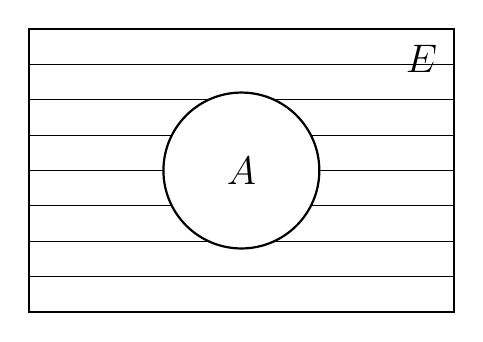
\begin{tikzpicture}[scale=0.45]
        \foreach \y in {1,...,7} {
            \draw (0,\y) -- (12,\y);
        }
        \draw[thick] (0,0) rectangle (12,8);
        
        \fill[white] (6,4) circle (2.2);
        \draw[thick] (6,4) circle (2.2);
        
        \node at (6,4) {\Large $A$};
        \node[anchor=north east] at (11.8, 7.8) {\Large $E$};
    \end{tikzpicture}
    \hspace{0.5cm}
    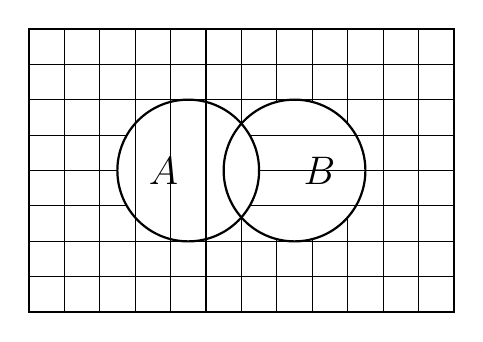
\begin{tikzpicture}[scale=0.45]
        \draw (0,0) grid (12,8);
        
        \fill[white] (4.5,4) circle (2);
        \fill[white] (7.5,4) circle (2);
        
        \begin{scope}
            \clip (4.5,4) circle (2);
            \foreach \x in {1,...,11} {
                \draw (\x,0) -- (\x,8);
            }
        \end{scope}
        
        \begin{scope}
            \clip (7.5,4) circle (2);
            \foreach \y in {1,...,7} {
                \draw (0,\y) -- (12,\y);
            }
        \end{scope}
        
        \begin{scope}
            \clip (4.5,4) circle (2);
            \fill[white] (7.5,4) circle (2);
        \end{scope}
        
        \draw[thick] (0,0) rectangle (12,8);
        \draw[thick] (4.5,4) circle (2);
        \draw[thick] (7.5,4) circle (2);
        
        \node at (3.8,4) {\Large $A$};
        \node at (8.2,4) {\Large $B$};
    \end{tikzpicture}
\end{center}

En la figura de la izquierda, \( A \) es un disco, contenido en el rectángulo, que es el conjunto fundamental \( E \). El complementario de \( A \) es la parte sombreada con líneas horizontales. En la figura de la derecha, \( A \) y \( B \) son discos. El complementario de \( A \) está sombreado con líneas horizontales y el complementario de \( B \) con líneas verticales. Entonces \( \mathcal{C}(A \cup B) \) es la parte cuadriculada, mientras que \( \mathcal{C}(A \cap B) \) es la parte que tiene algún tipo de línea (vertical, horizontal o ambas). Esto muestra que \( \mathcal{C}(A \cup B) = \mathcal{C}A \cap \mathcal{C}B \) y \( \mathcal{C}(A \cap B) = \mathcal{C}A \cup \mathcal{C}B \).

Otra operación útil entre conjuntos es el producto cartesiano. Se basa en el concepto de par ordenado, que discutiremos ahora.

Dados los objetos \( a, b \), el par ordenado \( (a, b) \) queda formado cuando se elige uno de esos objetos (a saber: \( a \)) para ser la primera coordenada del par y (consecuentemente) el objeto \( b \) para ser la segunda coordenada del par. Dos pares ordenados \( (a, b) \) y \( (a', b') \) serán llamados iguales cuando sus primeras coordenadas, \(a\) y \(a'\), sean iguales y sus segundas coordenadas, \(b\) y \(b'\), también. Así

\[
(a, b) = (a', b') \iff a = a' \text{ y } b = b'.
\]

No se debe confundir el par ordenado \((a, b)\) con el conjunto \(\{a, b\}\). En efecto, como dos conjuntos que poseen los mismos elementos son iguales, tenemos \(\{a, b\} = \{b, a\}\), sean cuales fueren \(a\) y \(b\). Por otro lado, por la definición de igualdad entre pares ordenados solo tenemos \((a, b) = (b, a)\) cuando \(a = b\). Notemos además que \(\{a, a\} = \{a\}\), mientras que \((a, a)\) es un par ordenado legítimo.

El producto cartesiano de los conjuntos \(A\) y \(B\) es el conjunto \(A \times B\) cuyos elementos son todos los pares ordenados \((a, b)\) cuya primera coordenada pertenece a \(A\) y la segunda a \(B\). Por tanto:

\[
A \times B = \{(a, b) \; ; \quad a \in A \text{ y } b \in B\}.
\]

Cuando \(A = B\), tenemos el producto cartesiano \(A^2 = A \times A\). El subconjunto \(\Delta \subset A \times A\), formado por los pares \((a, a)\) cuyas coordenadas son iguales, se llama la diagonal de \(A^2\).

\begin{center}
    \centering
    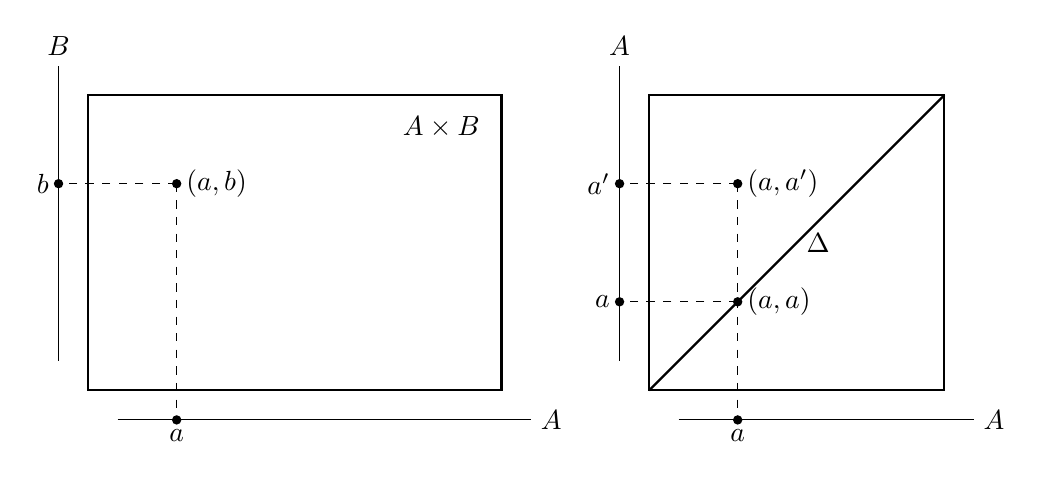
\begin{tikzpicture}[scale=0.75]

        \begin{scope}[shift={(0,0)}]
            \draw[thick] (0,0) rectangle (7,5);
            \node[anchor=north east] at (6.8, 4.8) {$A \times B$};

            \draw (-0.5, 0.5) -- (-0.5, 5.5);
            \node[anchor=south] at (-0.5, 5.5) {$B$};
            \draw (0.5, -0.5) -- (7.5, -0.5);
            \node[anchor=west] at (7.5, -0.5) {$A$};

            \node[circle, fill, inner sep=1.2pt] (a_axis_a) at (1.5, -0.5) {};
            \node[anchor=north] at (1.5, -0.5) {$a$};
            \node[circle, fill, inner sep=1.2pt] (a_axis_b) at (-0.5, 3.5) {};
            \node[anchor=east] at (-0.5, 3.5) {$b$};

            \node[circle, fill, inner sep=1.2pt] (a_pt) at (1.5, 3.5) {};
            \node[anchor=west] at (1.5, 3.5) {$(a,b)$};

            \draw[dashed] (1.5, 3.5) -- (1.5, -0.5);
            \draw[dashed] (1.5, 3.5) -- (-0.5, 3.5);
        \end{scope}

        \begin{scope}[shift={(9.5,0)}]
            \draw[thick] (0,0) rectangle (5,5);

            \draw (-0.5, 0.5) -- (-0.5, 5.5);
            \node[anchor=south] at (-0.5, 5.5) {$A$};
            \draw (0.5, -0.5) -- (5.5, -0.5);
            \node[anchor=west] at (5.5, -0.5) {$A$};

            \draw[thick] (0,0) -- (5,5);
            \node[anchor=west] at (2.5, 2.5) {$\Delta$};

            \node[circle, fill, inner sep=1.2pt] (b_axis_a_horiz) at (1.5, -0.5) {};
            \node[anchor=north] at (1.5, -0.5) {$a$};
            \node[circle, fill, inner sep=1.2pt] (b_axis_a_vert) at (-0.5, 1.5) {};
            \node[anchor=east] at (-0.5, 1.5) {$a$};
            \node[circle, fill, inner sep=1.2pt] (b_axis_aprime_vert) at (-0.5, 3.5) {};
            \node[anchor=east] at (-0.5, 3.5) {$a'$};

            \node[circle, fill, inner sep=1.2pt] (b_pt_aa) at (1.5, 1.5) {};
            \node[anchor=west] at (1.5, 1.5) {$(a,a)$};
            \node[circle, fill, inner sep=1.2pt] (b_pt_aap) at (1.5, 3.5) {};
            \node[anchor=west] at (1.5, 3.5) {$(a,a')$};

            \draw[dashed] (1.5, 3.5) -- (1.5, -0.5); 
            \draw[dashed] (1.5, 3.5) -- (-0.5, 3.5);
            \draw[dashed] (1.5, 1.5) -- (-0.5, 1.5);
        \end{scope}

    \end{tikzpicture}
\end{center}

En la figura de la izquierda, los conjuntos \(A\) y \(B\) están representados por segmentos y el producto cartesiano \(A \times B\) por un rectángulo. A la derecha, tenemos el cuadrado \(A \times A = A^2\), en el cual se destaca la diagonal \(\Delta\).

Ejemplo 8. Sean \(A = \{1, 2, 3\}\) y \(B = \{x, y\}\). Entonces  
\[A \times B = \{(1, x), (1, y), (2, x), (2, y), (3, x), (3, y)\}\]

Ejemplo 9. La introducción de coordenadas cartesianas en el plano hace que cada punto sea representado por un par ordenado \((x, y)\), donde \(x\) es su abscisa e \(y\) su ordenada. Esto identifica el plano con el producto cartesiano \(\mathbb{R}^2 = \mathbb{R} \times \mathbb{R}\), donde \(\mathbb{R}\) es el conjunto de los números reales.

\section{Funciones}

Una función \(f: A \to B\) consta de tres partes: un conjunto \(A\), llamado el dominio de la función (o el conjunto donde la función está definida), un conjunto \(B\), llamado el codominio de la función, o el conjunto donde la función toma valores, y una regla que permite asociar, de modo bien determinado, a cada elemento \(x \in A\), un único elemento \(f(x) \in B\), llamado el valor que la función asume en \(x\) (o en el punto \(x\)).

Se usa la notación \(x \mapsto f(x)\) para indicar que \(f\) hace corresponder a \(x\) el valor \(f(x)\).

Muchas veces se dice "la función \(f\)" en lugar de "la función \(f: A \to B\)". En este caso, quedan sobrentendidos el conjunto \(A\), dominio de \(f\), y el conjunto \(B\), codominio de \(f\).

No se debe confundir \(f\) con \(f(x)\): \(f\) es la función, mientras que \(f(x)\) es el valor que la función asume en un punto \(x\) de su dominio.

La naturaleza de la regla que enseña cómo obtener el valor \(f(x) \in B\) cuando se da \(x \in A\) es enteramente arbitraria, estando sujeta solo a dos condiciones:

\begin{enumerate}
\item No debe haber excepciones: para que \(f\) tenga el conjunto \(A\) como dominio, la regla debe proporcionar \(f(x)\) para todo \(x \in A\);

\item No debe haber ambigüedades: a cada \(x \in A\), la regla debe hacer corresponder un único \(f(x)\) en \(B\).
\end{enumerate}

Vemos que no existen funciones "plurívocas". Por la segunda condición, arriba, si \(x = y\) en \(A\), entonces \(f(x) = f(y)\) en \(B\).

Se deduce de las consideraciones anteriores que dos funciones \(f: A \to B\) y \(g: A' \to B'\) son iguales si, y solo si, \(A = A'\), \(B = B'\) y \(f(x) = g(x)\) para todo \(x \in A\). Es decir, dos funciones son iguales cuando tienen el mismo dominio, el mismo codominio y la misma regla de correspondencia.

Ejemplo 10. Sea \(P\) el conjunto de los polígonos del plano, \(\mathbb{R}\) el conjunto de los números reales y \(f: P \to \mathbb{R}\) la función que asocia a cada polígono \(x\) su área \(f(x)\).

Ejemplo 11. Sean \(A = B = \mathbb{Q}\). Intentemos definir una función \(f: \mathbb{Q} \to \mathbb{Q}\) considerando la siguiente regla: a cada número \(x \in \mathbb{Q}\), hagamos corresponder el número \(f(x) \in \mathbb{Q}\) tal que \(x \cdot f(x) = 1\). Esta regla no define una función de \(\mathbb{Q}\) en \(\mathbb{Q}\), pues dado \(0 \in \mathbb{Q}\), no existe número racional alguno \(y = f(0)\) tal que \(0 \cdot y = 1\). Sin embargo, si elegimos el conjunto \(A = \mathbb{Q} - \{0\}\) como dominio, la misma regla define la función \(f: A \to \mathbb{Q}\), \(f(x) = 1/x\).

Ejemplo 12. Sea \(T\) el conjunto de los triángulos del plano y \(\mathbb{R}^+\) el conjunto de los números reales positivos. Consideremos el intento de definir una función \(f: \mathbb{R}^+ \to T\) mediante la siguiente regla: a cada número real \(x > 0\) hagamos corresponder el triángulo \(f(x)\) cuya área es \(x\). Evidentemente, hay ambigüedades: dado un número real \(x > 0\), existe una infinidad de triángulos cuyo área es \(x\). La regla no define una función.

El gráfico de una función \(f: A \to B\) es el subconjunto \(G(f)\) del producto cartesiano \(A \times B\) formado por los pares ordenados \((x, f(x))\), donde \(x \in A\) es arbitrario. Es decir,

\[
G(f) = \{(x, y) \in A \times B \; ; \quad y = f(x)\}.
\]

Se sigue de la definición de igualdad entre funciones que dos funciones son iguales si, y solo si, poseen el mismo gráfico.

Para que un subconjunto \(G \subset A \times B\) sea el gráfico de una función \(f: A \to B\), es necesario y suficiente que, para cada \(x \in A\), exista un único punto \((x, y) \in G\) cuya primera coordenada sea \(x\). Para funciones \(f: A \to B\), donde \(A\) y \(B\) son conjuntos de números reales, esta condición significa que toda paralela al eje de las ordenadas, trazada por un punto de \(A\), debe cortar al gráfico \(G\) en uno y solo un punto.

\begin{center}
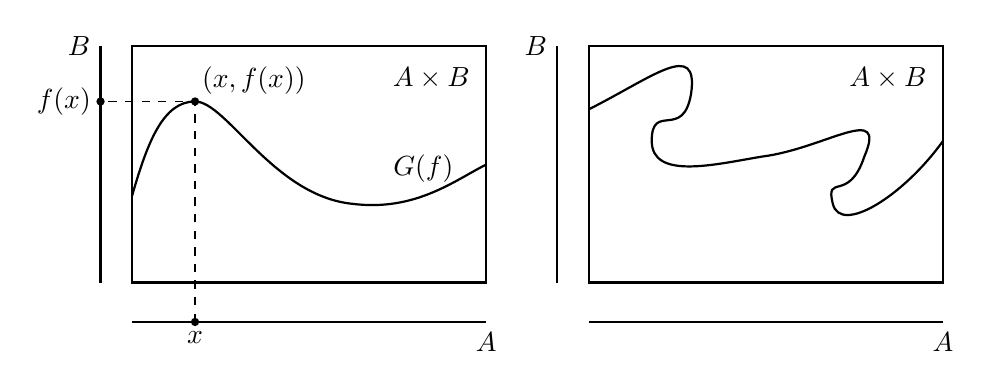
\begin{tikzpicture}

    \draw[thick] (0,0) rectangle (4.5, 3);
    \node at (3.8, 2.6) {$A \times B$};

    \draw[thick] (0,-0.5) -- (4.5,-0.5) node[below] {$A$};
    \draw[thick] (-0.4,0) -- (-0.4,3) node[left] {$B$};

    \draw[thick] (0, 1.1) .. controls (0.2, 1.8) and (0.4, 2.3) .. (0.8, 2.3)
                 .. controls (1.2, 2.3) and (1.8, 1.1) .. (2.8, 1.0)
                 .. controls (3.6, 0.9) and (4.1, 1.3) .. (4.5, 1.5);
                 
    \node at (3.7, 1.15) [above] {$G(f)$};

    \coordinate (x_val) at (0.8, -0.5);
    \coordinate (y_val) at (-0.4, 2.3);
    \coordinate (p_val) at (0.8, 2.3);

    \draw[dashed] (x_val) -- (p_val) -- (y_val);

    \fill (x_val) circle (1.5pt) node[below] {$x$};
    \fill (y_val) circle (1.5pt) node[left] {$f(x)$};
    \fill (p_val) circle (1.5pt) node[above right=-1pt] {$(x,f(x))$};

    \begin{scope}[xshift=5.8cm]

        \draw[thick] (0,0) rectangle (4.5, 3);
        \node at (3.8, 2.6) {$A \times B$};

        \draw[thick] (0,-0.5) -- (4.5,-0.5) node[below] {$A$};
        \draw[thick] (-0.4,0) -- (-0.4,3) node[left] {$B$};

        \draw[thick] (0,2.2)
                     .. controls (0.8, 2.6) and (1.4, 3.1) .. (1.3, 2.4)
                     .. controls (1.2, 1.8) and (0.8, 2.3) .. (0.8, 1.8)
                     .. controls (0.8, 1.3) and (1.6, 1.5) .. (2.2, 1.6)
                     .. controls (3.0, 1.7) and (3.8, 2.3) .. (3.5, 1.6)
                     .. controls (3.3, 1.0) and (3.0, 1.4) .. (3.1, 1.0)
                     .. controls (3.2, 0.6) and (4.0, 1.1) .. (4.5, 1.8);

    \end{scope}

\end{tikzpicture}
\end{center}

En la figura de la izquierda tenemos el gráfico de una función \(f: A \to B\). La figura de la derecha muestra un subconjunto de \(A \times B\) que no puede ser gráfico de una función de \(A\) en \(B\).

Una función \(f: A \to B\) se llama inyectiva (o biunívoca) cuando, dados \(x, y\) cualesquiera en \(A\), \(f(x) = f(y)\) implica \(x = y\). En otras palabras: cuando \(x \neq y\) en \(A\) implica \(f(x) \neq f(y)\) en \(B\).

El ejemplo más simple de una función inyectiva es la inclusión \(i: A \to B\), definida cuando \(A\) es un subconjunto de \(B\), por la regla \(i(x) = x\), para todo \(x \in A\).

Una función \(f: A \to B\) se llama sobreyectiva (o sobre \(B\)) cuando, para todo \(y \in B\) existe al menos un \(x \in A\) tal que \(f(x) = y\).

Ejemplos de funciones sobreyectivas son las proyecciones \(\pi_1: A \times B \to A\) y \(\pi_2: A \times B \to B\), de un producto cartesiano \(A \times B\) en los factores \(A\) y \(B\), respectivamente. La primera proyección, \(\pi_1\), se define por \(\pi_1(a, b) = a\), mientras que la segunda proyección, \(\pi_2\), se define por \(\pi_2(a, b) = b\).

Ejemplo 13. Sea \(f: \mathbb{Z} \to \mathbb{Z}\) definida por \(f(x) = x^2\). Entonces \(f\) no es inyectiva, pues \(f(-3) = f(3)\), aunque \(-3 \neq 3\). Tampoco \(f\) es sobreyectiva, pues no existe \(x \in \mathbb{Z}\) tal que \(x^2 = -1\). Por otro lado, si tomamos \(g: \mathbb{Z} \to \mathbb{Z}\), definida por \(g(x) = 3x + 1\), entonces \(g\) es inyectiva. De hecho, si \( g(x) = g(y) \) entonces \( 3x + 1 = 3y + 1 \), o sea, \( 3x = 3y \), de donde \( x = y \). Pero \( g \) no es sobreyectiva, pues no existe un entero \( x \) tal que \( 3x + 1 = 0 \), por ejemplo. Finalmente, sea \( h: \mathbb{N} \to \mathbb{N} \) definida así: \( h(1) = 1 \) y, para cada número natural \( x > 1 \), \( h(x) \) es el número de factores primos distintos que entran en la composición de \( x \). Entonces \( h \) es sobreyectiva, pues \( h(2) = 1 \), \( h(6) = 2 \), \( h(30) = 3 \), \( h(210) = 4 \), etc. Pero es claro que \( h \) no es inyectiva. Por ejemplo, si \( x \) e \( y \) son dos números primos cualesquiera, se tiene \( h(x) = h(y) \).

Ejemplo 14. La verificación de que una función es sobreyectiva implica demostrar la existencia de objetos que satisfacen ciertas condiciones. Por ejemplo, sea \( \mathbb{R}^+ \) el conjunto de los números reales positivos. Consideremos la función \( f: \mathbb{R} \to \mathbb{R}^+ \), definida por \( f(x) = x^2 \). Decir que \( f \) es sobreyectiva significa afirmar que, para todo número real \( y > 0 \) existe algún número real \( x \) tal que \( y = x^2 \), o sea, que todo número real positivo \( y \) posee una raíz cuadrada \( x \). (Esto será probado cuando estudiemos los números reales.) Otro ejemplo: sea \( p \) un polinomio no constante, de coeficientes complejos. A cada número complejo \( z \) asociemos el valor \( p(z) \) del polinomio \( p \). Esto define una función \( p: \mathbb{C} \to \mathbb{C} \), donde \( \mathbb{C} \) es el conjunto de los números complejos. La afirmación de que \( p \) es una función sobreyectiva es equivalente al llamado "Teorema Fundamental del Álgebra" (un teorema de Topología, según el cual todo polinomio complejo no constante posee al menos una raíz compleja). En efecto, admitiendo que \( p: \mathbb{C} \to \mathbb{C} \) es sobreyectiva, dado \( 0 \in \mathbb{C} \), debe existir algún \( z \in \mathbb{C} \) tal que \( p(z) = 0 \). El número \( z \) es, por tanto, una raíz de \( p \). Recíprocamente, admitiendo que todo polinomio no constante posee una raíz compleja, probamos que \( p: \mathbb{C} \to \mathbb{C} \) es sobreyectiva. En efecto, dado \( c \in \mathbb{C} \), la función \( z \mapsto p(z) - c \) es un polinomio no constante, luego existe algún \( z_0 \in \mathbb{C} \) tal que \( p(z_0) - c = 0 \). Se tiene \( p(z_0) = c \), de donde \( p \) es sobreyectiva.

Una función \( f: A \to B \) se llama biyectiva (una biyección, o una correspondencia biunívoca) cuando es inyectiva y sobreyectiva al mismo tiempo.

La más simple de las biyecciones es la función identidad \(\text{id}_A: A \to A\), definida por \(\text{id}_A(x) = x\), para todo \(x \in A\). Cuando no haya peligro de confusión, escribiremos simplemente \(\text{id}: A \to A\), en lugar de \(\text{id}_A\).

Por ejemplo, dados arbitrariamente \(a, b\) en \(\mathbb{Q}\), con \(a \neq 0\), la función \(f: \mathbb{Q} \to \mathbb{Q}\), definida por \(f(x) = ax + b\), es una biyección. En efecto, si \(f(x) = f(y)\), es decir, \(ax + b = ay + b\) entonces, sumando \(-b\) a ambos miembros, viene \(ax = ay\). Multiplicando ambos miembros por \(1/a\), obtenemos \(x = y\). Así, \(f\) es inyectiva. Además, dado \(y \in \mathbb{Q}\) cualquiera, el número racional \(x = (y - b)/a\) es tal que \(ax + b = y\), esto es, \(f(x) = y\), de donde \(f\) es sobreyectiva.

Dadas una función \(f: A \to B\) y una parte \(X \subset A\), se llama imagen de \(X\) por la función \(f\) al conjunto \(f(X)\) formado por los valores \(f(x)\) que \(f\) asume en los puntos \(x \in X\). Así

\[
f(X) = \{f(x) \; ; \quad x \in X\} = \{y \in B \; ; \quad y = f(x), \; x \in X\}.
\]

Evidentemente, \(f(X)\) es un subconjunto de \(B\). Para que \(f: A \to B\) sea sobreyectiva es necesario y suficiente que \(f(A) = B\). En general, se tiene solo \(f(A) \subset B\). El conjunto \(f(A)\) se llama la imagen de la función \(f\). A veces también se dice que \(f(A)\) es el conjunto de los valores de \(f\).

Dada una función \(f: A \to B\) e indicando con \(X, Y, \dots\) subconjuntos de \(A\), tenemos

I1) \(f(X \cup Y) = f(X) \cup f(Y)\),  \\
I2) \(f(X \cap Y) \subset f(X) \cap f(Y)\),  \\
I3) \(X \subset Y \Rightarrow f(X) \subset f(Y)\),  \\
I4) \(f(\emptyset) = \emptyset\).

Demostremos las dos primeras de estas relaciones.

I1) Si \(y \in f(X \cup Y)\), entonces existe \(x \in X \cup Y\) tal que \(f(x) = y\). Si \(x \in X\), tenemos \(y \in f(X)\). Si, en cambio, \(x \in Y\), tenemos \(y \in f(Y)\). En cualquier caso, \(y \in f(X) \cup f(Y)\). Luego \(f(X \cup Y) \subset f(X) \cup f(Y)\). Recíprocamente, sea \(z \in f(X) \cup f(Y)\). Entonces \(z \in f(X)\) o \(z \in f(Y)\). En el primer caso, existe \(x \in X\) tal que \(z = f(x)\). En el segundo, existe \(y \in Y\) tal que \(z = f(y)\). En cualquier hipótesis, existe \(w \in X \cup Y\) tal que \(z = f(w)\). Así \(z \in f(X \cup Y)\), esto es, \(f(X) \cup f(Y) \subset f(X \cup Y)\). Estas dos inclusiones muestran que \(f(X \cup Y) = f(X) \cup f(Y)\).

I2) Si \(y \in f(X \cap Y)\) entonces existe \(x \in X \cap Y\) tal que \(f(x) = y\). Entonces \(x \in X\) y por tanto \(y \in f(X)\). También \(x \in Y\) y por tanto \(y \in f(Y)\). Luego \(y \in f(X) \cap f(Y)\).

Ejemplo 15. Sea \(\mathbb{R}\) el conjunto de los números reales. Definimos \(f: \mathbb{R} \to \mathbb{R}\) poniendo \(f(x) = x^2\). Entonces la imagen de \(f\), o sea, el conjunto \(f(\mathbb{R})\), es el conjunto de los números reales \(\geq 0\). (Aquí estamos haciendo uso del hecho, que se demostrará más adelante, de que todo número real positivo posee una raíz cuadrada).

Ejemplo 16. Sea \(f: A \to B\) una función que no es inyectiva. Entonces existen \(x \neq y\) en \(A\), con \(f(x) = f(y)\). Pongamos \(X = \{x\}\) e \(Y = \{y\}\). Se tiene \(X \cap Y = \emptyset\), luego \(f(X \cap Y) = \emptyset\). Sin embargo \(f(X) \cap f(Y) = \{f(x)\}\) no es vacío. Luego, en este caso, tenemos \(f(X \cap Y) \neq f(X) \cap f(Y)\).

Si, en cambio, \(f: A \to B\) es inyectiva, podemos probar que \(f(X \cap Y) = f(X) \cap f(Y)\) para cualesquiera \(X, Y\) contenidos en \(A\).

En efecto, dado \(y \in f(X) \cap f(Y)\), tenemos \(y \in f(X)\) e \(y \in f(Y)\). Luego existen \(x' \in X\) y \(x'' \in Y\) con \(y = f(x')\) y \(y = f(x'')\). Como \(f\) es inyectiva, debe ser \(x' = x''\) y por tanto \(x' \in X \cap Y\). Se sigue que \(y = f(x')\) pertenece a \(f(X \cap Y)\), lo que muestra que \(f(X) \cap f(Y) \subset f(X \cap Y)\). Como la inclusión opuesta es siempre verdadera, concluimos que \(f(X \cap Y) = f(X) \cap f(Y)\).

En resumen, para que se tenga \(f(X \cap Y) = f(X) \cap f(Y)\) para cualesquiera \(X, Y\) contenidos en \(A\), es necesario y suficiente que la función \(f: A \to B\) sea inyectiva.

Dada una función \(f: A \to B\), consideremos un conjunto \(Y \subset B\). La imagen inversa de \(Y\) por la función \(f\) es el conjunto \(f^{-1}(Y)\), formado por todos los \(x \in A\) tales que \(f(x) \in Y\). Así:

\[
f^{-1}(Y) = \{x \in A \; ; \quad f(x) \in Y\}.
\]

Nótese que puede ocurrir \(f^{-1}(Y) = \emptyset\) incluso si \(Y \subset B\) es un subconjunto no vacío. Esto sucede precisamente cuando \(Y \cap f(A) = \emptyset\), es decir, cuando \(Y\) no tiene puntos en común con la imagen de \(f\). En particular, \(f\) no es sobreyectiva. Dado \(y \in B\), escribimos \(f^{-1}(y)\) en lugar de \(f^{-1}(\{y\})\). Puede ocurrir que \(f^{-1}(y)\) posea más de un elemento, pues \(f\) puede no ser inyectiva.

Ejemplo 17. Los subconjuntos del plano definidos en Geometría Analítica mediante ecuaciones y desigualdades son imágenes inversas de conjuntos. Por ejemplo, la recta que tiene la ecuación \(ax + by = c\) es el conjunto \(X = \{(x, y) \in \mathbb{R}^2 \; ; \quad ax + by = c\}\). Consideremos la función \(f: \mathbb{R}^2 \to \mathbb{R}\), definida por \(f(x, y) = ax + by\). Entonces la recta \(X\) es la imagen inversa del conjunto \(\{c\}\) por \(f\), o sea, \(X = f^{-1}(c)\). También la circunferencia cuya ecuación es \(x^2 + y^2 = 1\) (centro en el origen y radio 1) es el conjunto \(C = \{(x, y) \in \mathbb{R}^2 \; ; \quad x^2 + y^2 = 1\}\). Tomemos la función \(g: \mathbb{R}^2 \to \mathbb{R}\), definida por \(g(x, y) = x^2 + y^2\). Tenemos \(C = g^{-1}(1)\).

Ahora consideremos el disco \(D\) de centro en el origen y radio 1. Tenemos \(D = \{(x, y) \in \mathbb{R}^2 \; ; \quad x^2 + y^2 \leq 1\}\). Sea \(g: \mathbb{R}^2 \to \mathbb{R}\), nuevamente, la función definida por \(g(x, y) = x^2 + y^2\). Tomemos el intervalo \(I = [0, 1] = \{t \in \mathbb{R} \; ; \quad 0 \leq t \leq 1\}\). Entonces el disco \(D\) es la imagen inversa del intervalo \(I\) por la función \(g\): \(D = g^{-1}(I)\).

Las imágenes inversas se comportan bien relativamente a las operaciones con conjuntos. En la relación siguiente, \(Y\) y \(Z\) indican subconjuntos de \(B\). Dada una función \(f: A \to B\), tenemos

Inv1) \(f^{-1}(Y \cup Z) = f^{-1}(Y) \cup f^{-1}(Z)\),\\
Inv2) \(f^{-1}(Y \cap Z) = f^{-1}(Y) \cap f^{-1}(Z)\),\\
Inv3) \(f^{-1}(\mathcal{C}Y) = \mathcal{C} f^{-1}(Y)\),\\
Inv4) \(Y \subset Z \Rightarrow f^{-1}(Y) \subset f^{-1}(Z)\),\\
Inv5) \(f^{-1}(B) = A\),\\
Inv6) \(f^{-1}(\emptyset) = \emptyset\).

Vamos a demostrar las tres primeras.

Inv1) Tenemos \(x \in f^{-1}(Y \cup Z) \iff f(x) \in Y \cup Z \iff f(x) \in Y\) o \(f(x) \in Z \iff x \in f^{-1}(Y)\) o \(x \in f^{-1}(Z) \iff x \in f^{-1}(Y) \cup f^{-1}(Z)\).

Inv2) \(x \in f^{-1}(Y \cap Z) \iff f(x) \in Y \cap Z \iff f(x) \in Y\) y \(f(x) \in Z \iff x \in f^{-1}(Y)\) y \(x \in f^{-1}(Z) \iff x \in f^{-1}(Y) \cap f^{-1}(Z)\).

Inv3) \(x \in f^{-1}(\mathcal{C}Y) \iff f(x) \in \mathcal{C}Y \iff f(x) \notin Y \iff x \notin f^{-1}(Y) \iff x \in \mathcal{C} f^{-1}(Y)\).

\section{Composición de funciones}

Sean \(f: A \to B\) y \(g: B \to C\) funciones tales que el dominio de \(g\) es igual al codominio de \(f\). En este caso, podemos definir la función compuesta \(g \circ f: A \to C\), que consiste en aplicar primero \(f\) y después \(g\). Más precisamente,

\[
(g \circ f)(x) = g(f(x)) \quad \text{para todo } x \in A.
\]

Dadas \(f: A \to B\), \(g: B \to C\) y \(h: C \to D\), vale la ley asociativa
\[
(h \circ g) \circ f = h \circ (g \circ f): A \to D.
\]
En efecto, para todo \(x \in A\), tenemos:
\[
[(h \circ g) \circ f](x) = (h \circ g)(f(x)) = h[g(f(x))] = h[(g \circ f)(x)] = [h \circ (g \circ f)](x).
\]

Observamos que, más generalmente, basta que la imagen \(f(A)\) de la función \(f\) esté contenida en el dominio de \(g\) para que la definición \((g \circ f)(x) = g(f(x))\) tenga sentido y proporcione la función compuesta \(g \circ f: A \to C\).

Si \(f: A \to B\) y \(g: B \to C\) son inyectivas, entonces \(g \circ f: A \to C\) es inyectiva. También la compuesta de funciones sobreyectivas es sobreyectiva. En particular, la compuesta de dos biyecciones es una biyección. Estos hechos son de verificación inmediata.

Por otro lado, cualquier función \(f: A \to B\) puede escribirse como compuesta \(f = h \circ f_1\) de una función inyectiva \(h\) con una función sobreyectiva. Basta considerar \(f_1: A \to f(A)\), definida por \(f_1(x) = f(x)\), y la inclusión \(h: f(A) \to B\).

También podemos escribir cualquier función \(f: A \to B\) como compuesta \(f = \pi \circ F\) de una función sobreyectiva \(\pi\) con una función inyectiva \(F\). Basta tomar \(F: A \to A \times B\), donde \(F(x) = (x, f(x))\) y \(\pi: A \times B \to B\), con \(\pi(x, y) = y\) (segunda proyección).

Sean \(f: A \to B\) y \(g: B \to C\) funciones. Dado \(X \subset A\), se tiene \((g \circ f)(X) = g(f(X))\). Si \(Z \subset C\), tenemos \((g \circ f)^{-1}(Z) = f^{-1}(g^{-1}(Z))\).

Probemos esta última relación. Para \(x \in A\), tenemos:

\begin{align*}
x \in f^{-1}(g^{-1}(Z)) &\iff f(x) \in g^{-1}(Z) \\
&\iff g(f(x)) \in Z \\
&\iff (g \circ f)(x) \in Z \\
&\iff x \in (g \circ f)^{-1}(Z)
\end{align*}

La restricción de una función \(f: A \to B\) a un subconjunto \(X \subset A\) es la función \(f|_X: X \to B\), definida por \((f|_X)(x) = f(x)\) para todo \(x \in X\). Considerando la inclusión \(i: X \to A\), tenemos \(f|_X = f \circ i: X \to B\).

Dado \(X \subset A\), si \(g: X \to B\) es la restricción de una función \(f: A \to B\) al conjunto \(X\), se dice también que \(f\) es una extensión de \(g\). Extender una función \(g: X \to B\) al conjunto \(A \supset X\) es, por tanto, obtener una función \(f: A \to B\) que coincida con \(g\) en \(X\), esto es, tal que \(f|_X = g\). Evidentemente hay, en general, diversas extensiones de la misma función \(g\).

Un gran número de problemas matemáticos importantes se reducen a extender una o varias funciones de modo que las extensiones satisfagan ciertas condiciones adicionales (continuidad, analiticidad, etc.). La función que se desea extender se llama la "condición de contorno".

Dadas las funciones \(f: A \to B\) y \(g: B \to A\), diremos que \(g\) es una inversa a la izquierda para \(f\) cuando \(g \circ f = \text{id}_A: A \to A\), es decir, cuando \(g(f(x)) = x\) para todo \(x \in A\).

Por ejemplo, sean \(A\) el conjunto de los números reales \(\geq 0\) y \(\mathbb{R}\) el conjunto de todos los números reales. Consideremos \(f: A \to \mathbb{R}\), definida por \(f(x) = x^2\), y \(g: \mathbb{R} \to A\), definida por \(g(y) = \sqrt{y}\) si \(y \geq 0\) y \(g(y) = 0\) si \(y < 0\). Para todo \(x \in A\), tenemos \(g(f(x)) = g(x^2) = \sqrt{x^2} = x\). Luego \(g \circ f = \text{id}_A\) y, por tanto, \(g\) es una inversa a la izquierda de \(f\). Nótese que cualquier función \(h: \mathbb{R} \to A\), tal que \(h(y) = \sqrt{y}\) para \(y \geq 0\), es una inversa a la izquierda de \(f\). (La definición de los valores \(h(y)\) para \(y < 0\) puede ser cualquiera, sin que quede afectada la igualdad \(h \circ f = \text{id}_A\)).

Una función \(f: A \to B\) posee inversa a la izquierda si, y solo si, es inyectiva.

\textbf{Demostración}. Si \(f\) es inyectiva, para cada \(y \in f(A)\) existe un único \(x \in A\) tal que \(y = f(x)\). Escribamos \(x = g(y)\). Esto define una función \(g: f(A) \to A\) tal que \(g(f(x)) = x\) para todo \(x \in A\). Completamos la definición de \(g: B \to A\) poniendo, por ejemplo, \(g(y) = x_0\) (elemento que fijamos en \(A\)) para \(y \in B - f(A)\). Obtenemos \(g: B \to A\) tal que \(g \circ f = \text{id}_A\). Recíprocamente, si existe \(g: B \to A\) tal que \(g \circ f = \text{id}_A\) entonces, dados \(x', x''\) en \(A\), \(f(x') = f(x'') \Rightarrow x' = g(f(x')) = g(f(x'')) = x''\), y por tanto, \(f\) es inyectiva.

Una función \(g: B \to A\) se llama inversa a la derecha de una función \(f: A \to B\) cuando \(f \circ g = \text{id}_B: B \to B\), es decir, cuando \(f(g(y)) = y\) para todo \(y \in B\).

Por ejemplo, sea \(f: \mathbb{N} \to \mathbb{N}\) definida por \(f(1) = 1\) y, si \(x > 1\), \(f(x) =\) número de factores primos distintos que entran en la composición de \(x\). Definamos \(g: \mathbb{N} \to \mathbb{N}\) poniendo \(g(y) =\) menor número natural que es el producto de \(y\) factores primos distintos. Entonces, para todo número natural \(y\), tenemos \(f(g(y)) = y\). Luego \(f \circ g = \text{id}_{\mathbb{N}}\) y, por tanto, \(g\) es una inversa a la derecha para \(f\). Otras funciones \(h: \mathbb{N} \to \mathbb{N}\) podrían definirse con la propiedad \(f \circ h = \text{id}_{\mathbb{N}}\). Por ejemplo, podríamos poner \(h(y) =\) menor número natural divisible por 13 que es el producto de \(y\) factores primos distintos.

Una función \(f: A \to B\) posee inversa a la derecha si, y solo si, es sobreyectiva.

\textbf{Demostración}. Sea \(f: A \to B\) sobreyectiva. Entonces, para cada \(y \in B\), el conjunto \(f^{-1}(y)\) no es vacío. Elijamos, para cada \(y \in B\), un \(x \in A\) tal que \(f(x) = y\) y pongamos \(g(y) = x\). Esto define una función \(g: B \to A\) tal que \(f(g(y)) = y\). Luego \(g\) es una inversa a la derecha de \(f\). Recíprocamente, si existe \(g: B \to A\) con \(f \circ g = \text{id}_B\) entonces, para cada \(y \in B\), poniendo \(x = g(y)\), tenemos \(f(x) = f(g(y)) = y\). Luego \(f\) es sobreyectiva.

Una función \(g: B \to A\) se llama inversa de la función \(f: A \to B\) cuando \(g \circ f = \text{id}_A\) y \(f \circ g = \text{id}_B\), es decir, cuando \(g\) es inversa a izquierda y a la derecha para \(f\).

Por ejemplo, sea \(a\) un número racional \(\neq 0\) y definamos \(f: \mathbb{Q} \to \mathbb{Q}\) poniendo \(f(x) = ax\). La función \(g: \mathbb{Q} \to \mathbb{Q}\), definida por \(g(x) = x/a\), es inversa de \(f\).

Otro ejemplo: dada una función arbitraria \(f: A \to B\), sea \(G(f)\) el gráfico de \(f\). (Recordemos que \(G(f)\) es el subconjunto de \(A \times B\) formado por los pares ordenados \((x, f(x))\), donde \(x\) recorre \(A\).) Definimos una función \(F: A \to G(f)\) poniendo \(F(x) = (x, f(x))\). Sea \(\pi: G(f) \to A\) definida por \(\pi(x, f(x)) = x\). (Evidentemente, \(\pi = \pi_1 |_{G(f)}\) es la restricción a \(G(f)\) de la primera proyección \(\pi_1: A \times B \to A\).) Entonces \(F \circ \pi = \text{id}_{G(f)}\) y \(\pi \circ F = \text{id}_A\), como se ve fácilmente. Por tanto \(\pi\) es inversa de \(F\).

Se sigue de las dos proposiciones anteriores que una función \(f: A \to B\) posee inversa si, y solo si, es una biyección.

Al contrario de las inversas de un solo lado, si una función \(f: A \to B\) posee una inversa, ella es única.

En efecto, supongamos que \(g: B \to A\) y \(h: B \to A\) sean ambas inversas de \(f\). Entonces \(h = h \circ \text{id}_B = h \circ (f \circ g) = (h \circ f) \circ g = \text{id}_A \circ g = g\).

El lector atento habrá notado que probamos arriba un poco más de lo enunciado, a saber: si \(f\) posee una inversa a la izquierda, \(h\), y una inversa a la derecha, \(g\), entonces \(h = g\) y \(f\) tiene una inversa.

Escribiremos \(f^{-1}: B \to A\) para indicar la inversa de la biyección \(f: A \to B\).

Evidentemente, si \(f: A \to B\) y \(g: B \to C\) son biyecciones, se tiene \((g \circ f)^{-1} = f^{-1} \circ g^{-1}\).

\section{Familias}

Una familia es una función cuyo valor en un punto \(x\) se indica con \(f_x\) en lugar de \(f(x)\).

Pasemos a las definiciones formales.
Sea \(L\) un conjunto, cuyos elementos llamaremos índices y representaremos genéricamente por \(\lambda\).

Dado un conjunto \(X\), una familia de elementos de \(X\) con índices en \(L\) es una función \(x: L \to X\). El valor de \(x\) en el punto \(\lambda \in L\) se indicará con el símbolo \(x_\lambda\), en lugar de la notación usual \(x(\lambda)\). La familia \(x\) se representa por la notación \((x_\lambda)_{\lambda \in L}\) o simplemente \((x_\lambda)\) cuando no haya duda sobre el conjunto de índices \(L\).

Tomemos, por ejemplo, \(L = \{1, 2\}\) como conjunto de índices. Dado un conjunto \(X\), una familia de elementos de \(X\) con índices en \(L\) es una función \(x: \{1, 2\} \to X\). Los valores de esta función en los puntos 1 y 2 se representan por \(x_1\) y \(x_2\). Se obtiene así un par ordenado \((x_1, x_2)\) de elementos de \(X\). Recíprocamente, todo par ordenado \((x_1, x_2)\) de elementos de \(X\) es una familia \(x: \{1, 2\} \to X\). En suma, los pares ordenados de elementos de \(X\) son las familias de elementos de \(X\) con índices en el conjunto \(L = \{1, 2\}\). Es decir, el producto cartesiano \(X^2 = X \times X\) es el conjunto de las funciones (familias) \(x: \{1, 2\} \to X\). Más generalmente, dados los conjuntos \(X_1\) y \(X_2\), el producto cartesiano \(X_1 \times X_2\) es el conjunto de las familias \(x: \{1, 2\} \to X_1 \cup X_2\) tales que \(x_1 \in X_1\) y \(x_2 \in X_2\).

Cuando \(L = \{1, 2, \dots, n\}\) es el conjunto de los números naturales desde 1 hasta \(n\), una familia \(x: L \to X\) se llama una \(n\)-upla de elementos de \(X\). Una \(n\)-upla \(x = (x_i)_{i \in L}\) se representa comúnmente por la notación \(x = (x_1, \dots, x_n)\). El elemento \(x_i\) se llama la \(i\)-ésima coordenada de la \(n\)-upla \(x = (x_1, \dots, x_n)\).

Sea \((A_\lambda)_{\lambda \in L}\) una familia de conjuntos con índices en \(L\). (Esto quiere decir: a cada \(\lambda \in L\) hacemos corresponder un conjunto \(A_\lambda\).) La unión de esa familia es el conjunto de los elementos que pertenecen al menos a uno de los conjuntos \(A_\lambda\). Se representa por la notación \(\bigcup_{\lambda \in L} A_\lambda\) o, simplemente, \(\bigcup A_\lambda\). Así

\[
\bigcup_{\lambda \in L} A_\lambda = \{x \; ; \quad \text{existe } \lambda \in L \text{ con } x \in A_\lambda\}.
\]

En otras palabras, \(\bigcup A_\lambda\) es el conjunto de los elementos que pertenecen a algún \(A_\lambda\).

Análogamente, la intersección de la familia \((A_\lambda)_{\lambda \in L}\) es el conjunto de los elementos que pertenecen simultáneamente a todos los \(A_\lambda\).

Notación: \(\bigcap_{\lambda \in L} A_\lambda\) o simplemente \(\bigcap A_\lambda\). Por tanto,

\[
\bigcap_{\lambda \in L} A_\lambda = \{x \; ; \quad x \in A_\lambda \text{ para todo } \lambda \in L\}.
\]

Cuando \(L = \{1, 2, \dots, n\}\), se escribe

\[
\bigcup_{i \in L} A_i = \bigcup_{i=1}^n A_i = A_1 \cup \cdots \cup A_n,
\]
\[
\bigcap_{i \in L} A_i = \bigcap_{i=1}^n A_i = A_1 \cap \cdots \cap A_n.
\]

Una familia con índices en el conjunto \(\mathbb{N} = \{1, 2, \dots\}\) de los números naturales se llama una sucesión. Así, una sucesión \(x = (x_n)_{n \in \mathbb{N}} = (x_1, x_2, \dots, x_n, \dots)\) de elementos de un conjunto \(X\) es una función \(x: \mathbb{N} \to X\), donde el valor \(x(n)\) se indica con el símbolo \(x_n\) y se llama el n-ésimo término de la sucesión.

Dada una sucesión de conjuntos \((A_n)_{n \in \mathbb{N}}\), su unión y su intersección se representan por

\[
\bigcup_{n \in \mathbb{N}} A_n = \bigcup_{n=1}^\infty A_n = A_1 \cup A_2 \cup \cdots \cup A_n \cup \cdots,
\]
\[
\bigcap_{n \in \mathbb{N}} A_n = \bigcap_{n=1}^\infty A_n = A_1 \cap A_2 \cap \cdots \cap A_n \cap \cdots.
\]

Ejemplo 18. Para cada \(n \in \mathbb{N}\), consideremos el conjunto

\[
A_n = \{-n, -n+1, \dots, -1, 0, 1, \dots, n-1, n\}.
\]

Entonces

\[
\bigcup_{n=1}^\infty A_n = \mathbb{Z} \quad \text{y} \quad \bigcap_{n=1}^\infty A_n = \{-1, 0, 1\},
\]

como se ve fácilmente.

Dada una familia \((A_\lambda)_{\lambda \in L}\) de subconjuntos de un conjunto fundamental \(E\), se tiene

\[
\mathcal{C}\left(\bigcup A_\lambda\right) = \bigcap \mathcal{C} A_\lambda
\]

y

\[
\mathcal{C}\left(\bigcap A_\lambda\right) = \bigcup \mathcal{C} A_\lambda.
\]

En efecto, dado \(x \in E\), tenemos sucesivamente \(x \in \mathcal{C}(\bigcup A_\lambda) \iff x \notin \bigcup A_\lambda \iff\) no existe \(\lambda \in L\) tal que \(x \in A_\lambda \iff x \notin A_\lambda\) para todo \(\lambda \in L \iff x \in \mathcal{C} A_\lambda\) para todo \(\lambda \in L \iff x \in \bigcap \mathcal{C} A_\lambda\).

Esto prueba la primera igualdad. La segunda es consecuencia, teniendo en cuenta que \(\mathcal{C}(\mathcal{C}X) = X\). En efecto, si escribimos \(\mathcal{C} A_\lambda = B_\lambda\), tenemos \(\mathcal{C} B_\lambda = A_\lambda\). Luego

\[
\mathcal{C}\left(\bigcap A_\lambda\right) = \mathcal{C}\left(\bigcap \mathcal{C} B_\lambda\right) = \mathcal{C}\left(\mathcal{C}\left(\bigcup B_\lambda\right)\right) = \bigcup B_\lambda = \bigcup \mathcal{C} A_\lambda.
\]

Ejemplo 19. Sea \((A_\lambda)_{\lambda \in L}\) una familia de subconjuntos de un conjunto \(E\). Afirmar que \(\bigcup A_\lambda = E\) equivale a decir que, para todo elemento \(x \in E\) existe al menos un \(\lambda \in L\) tal que \(x \in A_\lambda\). Sea \(B_\lambda = \mathcal{C} A_\lambda\). Se tiene \(\bigcup A_\lambda = E\) si, y solo si, la intersección de los \(B_\lambda\) es vacía, esto es, \(\bigcap B_\lambda = \emptyset\). En efecto, por lo que vimos \(\bigcap B_\lambda = \mathcal{C}(\bigcup A_\lambda)\).

Dada una función \(f: A \to B\), consideremos una familia \((A_\lambda)_{\lambda \in L}\) de subconjuntos de \(A\), y una familia \((B_\mu)_{\mu \in M}\) de subconjuntos de \(B\). Se tiene

\[
f\left(\bigcup A_\lambda\right) = \bigcup f(A_\lambda),
\]
\[
f\left(\bigcap A_\lambda\right) \subset \bigcap f(A_\lambda),
\]
\[
f^{-1}\left(\bigcup B_\mu\right) = \bigcup f^{-1}(B_\mu),
\]
\[
f^{-1}\left(\bigcap B_\mu\right) = \bigcap f^{-1}(B_\mu).
\]

Probemos la primera y la última de estas afirmaciones. Dado \(y \in B\), tenemos:

\[
y \in f\left(\bigcup A_\lambda\right) \iff \text{existe } x \in \bigcup A_\lambda \text{ tal que } y = f(x)
\]
\[
\iff \text{existen } \lambda \in L \text{ y } x \in A_\lambda \text{ con } y = f(x)
\]
\[
\iff \text{existe } \lambda \in L \text{ tal que } y \in f(A_\lambda)
\]
\[
\iff y \in \bigcup f(A_\lambda).
\]

Dado \( x \in A \), tenemos

\[
x \in f^{-1}(\cap B_\mu) \iff f(x) \in \cap B_\mu \iff f(x) \in B_\mu \text{ para todo } \mu \in M
\]
\[
\iff x \in f^{-1}(B_\mu) \text{ para todo } \mu \in M \iff x \in \cap f^{-1}(B_\mu).
\]

La noción de familia permite considerar productos cartesianos de una cantidad arbitraria de conjuntos.

Dados los conjuntos \( A_1, \ldots, A_n \), su producto cartesiano

\[
A = A_1 \times \cdots \times A_n = \prod_{i=1}^n A_i
\]

es el conjunto formado por todas las \( n \)-uplas \( a = (a_1, \ldots, a_n) \) tales que \( a_1 \in A_1, \ldots, a_n \in A_n \).

En otras palabras, \( A_1 \times \cdots \times A_n \) es el conjunto de todas las funciones \( a : \{1, 2, \ldots, n\} \to A_1 \cup A_2 \cup \cdots \cup A_n \) tales que \( a(i) = a_i \in A_i \) para \( i = 1, 2, \ldots, n \).

Esta definición extiende la del producto cartesiano \( A \times B \).

Cuando \( A_1 = \cdots = A_n = A \), el producto cartesiano \( A \times \cdots \times A \) de \( n \) copias de \( A \) se indica con \( A^n \). Consiste en todas las funciones \( a : \{1, 2, \ldots, n\} \to A \), es decir, de todas las \( n \)-uplas de elementos de \( A \).

En el producto cartesiano \( A = A_1 \times \cdots \times A_n \), destacan las proyecciones \( \pi_1 : A \to A_1 \), \( \pi_2 : A \to A_2, \ldots, \pi_n : A \to A_n \). La \( i \)-ésima proyección \( \pi_i : A \to A_i \) se define poniendo \( \pi_i(a) = a_i = i \)-ésima coordenada de la \( n \)-upla \( a = (a_1, \ldots, a_n) \). Dados \( a = (a_1, \ldots, a_n) \) y \( b = (b_1, \ldots, b_n) \) en \( A_1 \times \cdots \times A_n \), se tiene \( a = b \) si, y solo si, \( \pi_i(a) = \pi_i(b) \) para cada \( i = 1, \ldots, n \).

Sea \( X \subset A_1 \times \cdots \times A_n \). Los elementos \( x = (x_1, \ldots, x_n) \) de \( X \) poseen \( n \) coordenadas. Las funciones \( f : X \to B \), definidas en \( X \), pueden ser pensadas como funciones de \( n \) variables (la primera variable estando en \( A_1 \), la segunda en \( A_2 \), etc.) En particular, introduciendo coordenadas cartesianas en el plano, este se identifica con el producto cartesiano \( \mathbb{R}^2 = \mathbb{R} \times \mathbb{R} \). Las funciones \( f : X \to \mathbb{R} \), definidas en subconjuntos \( X \subset \mathbb{R}^2 \), son las funciones reales de dos variables reales.

Dada una familia de conjuntos \( (A_\lambda)_{\lambda \in L} \), su producto cartesiano

\[
A = \prod_{\lambda \in L} A_\lambda
\]

es el conjunto de las familias \((a_\lambda)_{\lambda \in L}\) tales que, para cada \(\lambda \in L\), se tiene \(a_\lambda \in A_\lambda\).

En otras palabras, \(A\) es el conjunto de todas las funciones \(a: L \to \bigcup A_\lambda\) tales que \(a(\lambda) = a_\lambda \in A_\lambda\) para cada \(\lambda \in L\).

Las proyecciones \(\pi_\lambda: A \to A_\lambda\) se definen por \(\pi_\lambda(a) = a_\lambda\). Cada proyección \(\pi_\lambda\) es una función sobreyectiva. Dada una función \(f: X \to \prod A_\lambda\), de un conjunto cualquiera \(X\) en el producto cartesiano de los \(A_\lambda\), se obtiene, para cada \(\lambda \in L\), una función \(f_\lambda: X \to A_\lambda\), dada por \(f_\lambda = \pi_\lambda \circ f\). Así, \(f(x) = (f_\lambda(x))_{\lambda \in L}\) para cada \(x \in X\). Recíprocamente, si se da, para cada \(\lambda \in L\), una función \(f_\lambda: X \to A_\lambda\), entonces existe una única \(f: X \to \prod A_\lambda\) tal que \(f_\lambda = \pi_\lambda \circ f\) para cada \(\lambda \in L\). Basta poner \(f(x) = (f_\lambda(x))_{\lambda \in L}\) para cada \(x \in X\). Las funciones \(f_\lambda\) se llaman las coordenadas de \(f\).

En el caso particular en que todos los conjuntos \(A_\lambda\) son iguales al mismo conjunto \(A\), se escribe \(A^L\) en lugar de \(\prod_{\lambda \in L} A_\lambda\). \(A^L\) es, por tanto, el conjunto de todas las funciones de \(L\) en \(A\).

Se destaca, en especial, el producto cartesiano de una sucesión de conjuntos \(A_1, A_2, \dots, A_n, \dots\), el cual se representa con las notaciones

\[
\prod_{n \in \mathbb{N}} A_n = \prod_{n=1}^{\infty} A_n = A_1 \times A_2 \times \cdots \times A_n \times \dots
\]

Los elementos de este conjunto son las sucesiones \(a = (a_1, a_2, \dots, a_n, \dots)\) sujetas a la condición de que \(a_n \in A_n\) para todo \(n \in \mathbb{N}\).

\textbf{Ejercicios}

1. Dados los conjuntos \(A\) y \(B\), sea \(X\) un conjunto con las siguientes propiedades:

\begin{itemize}
\item[] \(1^\text{a}\) \(X \supset A\) y \(X \supset B\),
\item[] \(2^\text{a}\) Si \(Y \supset A\) y \(Y \supset B\) entonces \(Y \supset X\).
\end{itemize}

Probar que \(X = A \cup B\).

2. Enuncie y demuestre un resultado análogo al anterior, caracterizando \( A \cap B \).

3. Sean \( A, B \subset E \). Pruebe que \( A \cap B = \emptyset \) si, y solo si, \( A \subset \mathcal{C}B \). Pruebe también que \( A \cup B = E \) si, y solo si, \( \mathcal{C}A \subset B \).

4. Dados \( A, B \subset E \), pruebe que \( A \subset B \) si, y solo si, \( A \cap \mathcal{C}B = \emptyset \).

5. Dé ejemplo de conjuntos \( A, B, C \) tales que \( (A \cup B) \cap C \neq A \cup (B \cap C) \).

6. Si \( A, X \subset E \) son tales que \( A \cap X = \emptyset \) y \( A \cup X = E \), pruebe que \( X = \mathcal{C}A \).

7. Si \( A \subset B \), entonces \( B \cap (A \cup C) = (B \cap C) \cup A \) para todo conjunto \( C \). Por otro lado, si existe \( C \) de modo que la igualdad anterior sea satisfecha, entonces \( A \subset B \).

8. Pruebe que \( A = B \) si, y solo si, \( (A \cap \mathcal{C}B) \cup (\mathcal{C}A \cap B) = \emptyset \).

9. Pruebe que \( (A - B) \cup (B - A) = (A \cup B) - (A \cap B) \).

10. Sea \( A \Delta B = (A - B) \cup (B - A) \). Pruebe que \( A \Delta B = A \Delta C \) implica \( B = C \). Examine la validez de un resultado análogo con \( \cap, \cup \) o \( \times \) en lugar de \( \Delta \).

11. Pruebe las siguientes afirmaciones:

a) \( (A \cup B) \times C = (A \times C) \cup (B \times C) \);\\
b) \( (A \cap B) \times C = (A \times C) \cap (B \times C) \);\\
c) \( (A - B) \times C = (A \times C) - (B \times C) \);\\
d) \( A \subset A', B \subset B' \Rightarrow A \times B \subset A' \times B' \).

12. Dada la función \( f: A \to B \):

a) Pruebe que se tiene \( f(X - Y) \supset f(X) - f(Y) \), sean cuales fueren los subconjuntos \( X \) e \( Y \) de \( A \);\\
b) Muestre que si \(f\) es inyectiva entonces \(f(X - Y) = f(X) - f(Y)\) para cualesquiera \(X, Y\) contenidos en \(A\).

13. Muestre que la función \(f: A \to B\) es inyectiva si, y solo si, \(f(A - X) = f(A) - f(X)\) para todo \(X \subset A\).

14. Dada la función \(f: A \to B\), pruebe:

a) \(f^{-1}(f(X)) \supset X\) para todo \(X \subset A\);\\
b) \(f\) es inyectiva si, y solo si, \(f^{-1}(f(X)) = X\) para todo \(X \subset A\).

15. Dada \(f: A \to B\), pruebe:

a) para todo \(Z \subset B\), se tiene \(f(f^{-1}(Z)) \subset Z\);\\
b) \(f\) es sobreyectiva si, y solo si, \(f(f^{-1}(Z)) = Z\) para todo \(Z \subset B\).

16. Dada una familia de conjuntos \((A_\lambda)_{\lambda \in L}\), sea \(X\) un conjunto con las siguientes propiedades:

\begin{itemize}
\item[] 1ª) para todo \(\lambda \in L\), se tiene \(X \supset A_\lambda\);

\item[] 2ª) Si \(Y \supset A_\lambda\) para todo \(\lambda \in L\), entonces \(Y \supset X\).
\end{itemize}

Pruebe que, en estas condiciones, se tiene \(X = \bigcup_{\lambda \in L} A_\lambda\).

17. Enuncie y demuestre un resultado análogo al anterior, caracterizando \(\bigcap_{\lambda \in L} A_\lambda\).

18. Sea \(f: \mathcal{P}(A) \to \mathcal{P}(A)\) una función tal que \(X \subset Y \Rightarrow f(Y) \subset f(X)\) y \(f(f(X)) = X\). Pruebe que \(f(\bigcup X_\lambda) = \bigcap f(X_\lambda)\) y \(f(\bigcap X_\lambda) = \bigcup f(X_\lambda)\). [Aquí \(X, Y\) y cada \(X_\lambda\) son subconjuntos de \(A\)].

19. Dadas las familias \((A_\lambda)_{\lambda \in L}\) y \((B_\mu)_{\mu \in M}\), forme dos familias con índices en \(L \times M\) considerando los conjuntos
\[
(A_\lambda \cup B_\mu)_{(\lambda, \mu) \in L \times M} \quad \text{y} \quad (A_\lambda \cap B_\mu)_{(\lambda, \mu) \in L \times M}.
\]
Pruebe que se tiene

\[
\left( \bigcup_{\lambda \in L} A_\lambda \right) \cap \left( \bigcup_{\mu \in M} B_\mu \right) = \bigcup_{(\lambda,\mu) \in L \times M} (A_\lambda \cap B_\mu),
\]
\[
\left( \bigcap_{\lambda \in L} A_\lambda \right) \cup \left( \bigcap_{\mu \in M} B_\mu \right) = \bigcap_{(\lambda,\mu) \in L \times M} (A_\lambda \cup B_\mu).
\]

20. Sea \((A_{ij})_{(i,j) \in \mathbb{N} \times \mathbb{N}}\) una familia de conjuntos con índices en \(\mathbb{N} \times \mathbb{N}\). Pruebe, o refute mediante un contraejemplo, la igualdad

\[
\bigcup_{j=1}^{\infty} \left( \bigcap_{i=1}^{\infty} A_{ij} \right) = \bigcap_{i=1}^{\infty} \left( \bigcup_{j=1}^{\infty} A_{ij} \right).
\]

21. Dados los conjuntos \(A, B, C\), establezca una biyección entre \(\mathcal{F}(A \times B; C)\) y \(\mathcal{F}(A; \mathcal{F}(B; C))\).
